\section{Experiments}

We implement Algorithm~\ref{alg:sigma} for calibrating a noise multiplier for a given mechanism under balls-in-bins batching. In this section, we look at both the problem of minimizing RMSE and a deep learning setting, and compare results enabled by our accounting and optimization routines to past work.

For all our empirical results, we use $\delta = 8 \cdot 10^{-6}, \tau = 1.25, s = 10^8$. For this set of values, Theorem~\ref{thm:bernstein} gives a failure probability less than $7.2 \cdot 10^{-9}$. We use Algorithm~\ref{alg:wrapper} to verify the DP guarantee for both the add and remove adjacencies, but by a union bound the failure probability increases to at most $1.5 \cdot 10^{-8}$ once accounting for both adjacencies, much smaller than $\tau \delta = 10^{-5}$. So, we can apply Theorem~\ref{thm:wrapper} to show $(\epsilon, 10^{-5})$-DP for all our empirical results.

\newcommand{\defaultgraphics}[1]{\includegraphics[width=\textwidth]{#1}}

\subsection{RMSE Results}


\subsubsection{Analysis of the amplification schemes}

We first focus on the RMSE metric $\sigma \cdot \|\bfA^{-1} \bfC\|$. We compare our balls-in-bins batching analysis, Poisson sampling (using the analysis of \citep{choquette2024amplified} for $b$-banded matrices where $b > 1$, and standard PLD accounting for DP-SGD), and no amplification (i.e., we do multiple passes using a fixed batch size over a dataset given in arbitrary order). To simplify presentation in this section we will restrict to the setting with 2048 total iterations and 16 epochs, i.e. 128 iterations per epoch or $B = |D|/128$. In Appendix~\ref{sec:other-settings}, we provide analogous results for other settings of the number of epochs and number of iterations per epoch; while the exact numbers differ in other settings, the high-level conclusions hold in all settings we tested.

\mypar{Amplification of DP-SGD} In \cref{fig:improvement-on-dpsgd}, we plot the percentage improvement in RMSE due to balls-in-bins and Poisson sampling over the unamplified RMSE of DP-SGD, i.e. $\bfC = \bfI$.

\begin{figure}
\centering
\begin{subfigure}{.45\textwidth}
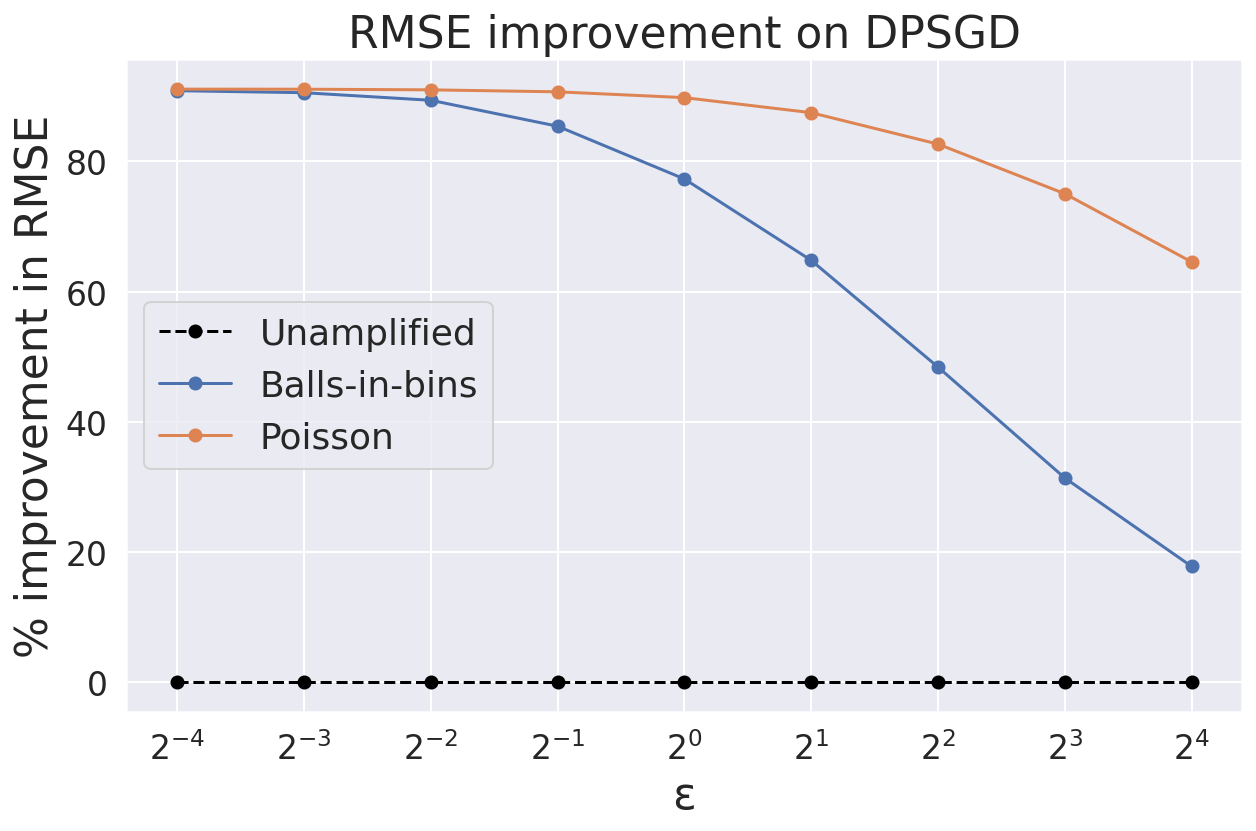
\includegraphics[width=0.95\linewidth]{other_figures/improvement-on-dp-sgd.png}
\caption{Improvement in RMSE over unamplified DP-SGD due to different amplification schemes.}
\label{fig:improvement-on-dpsgd}
\end{subfigure}
\begin{subfigure}{.05\textwidth}
\end{subfigure}
\begin{subfigure}{.45\textwidth}
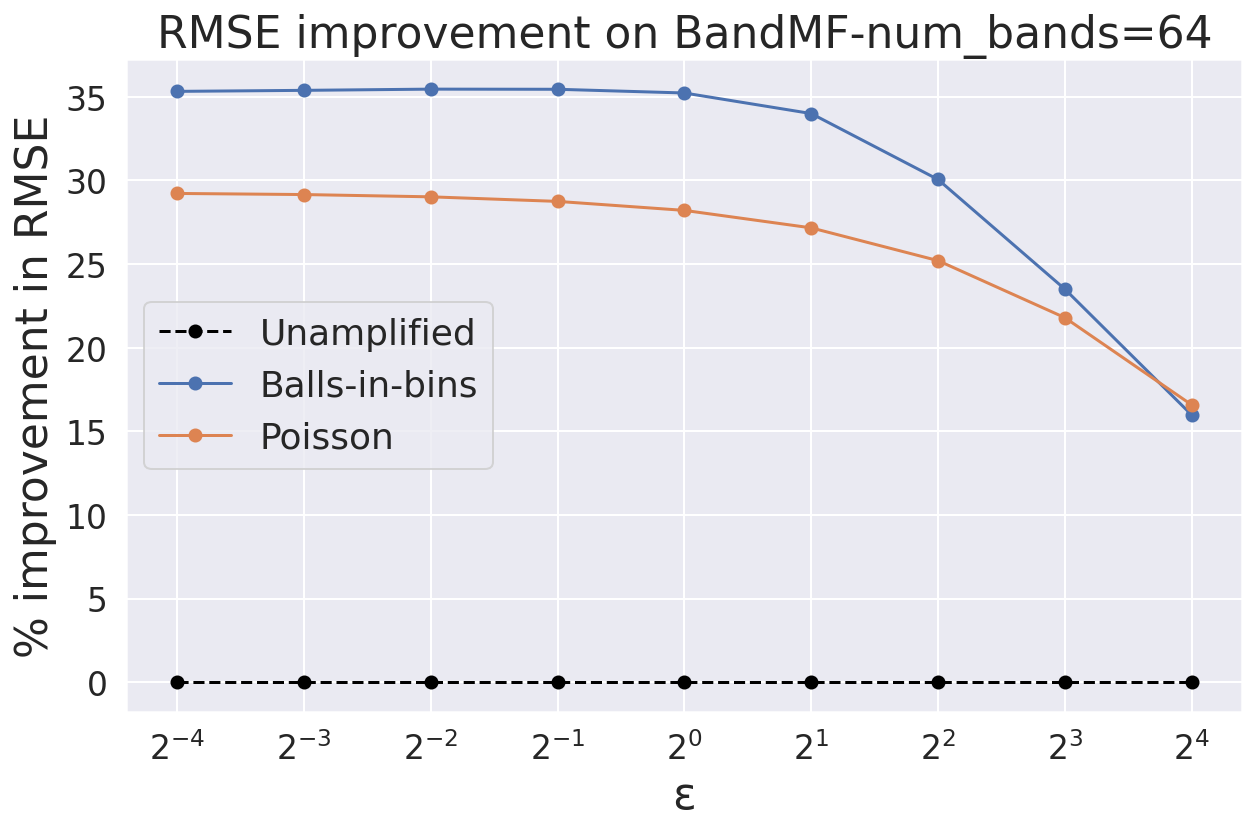
\includegraphics[width=0.95\linewidth]{other_figures/improvement-on-band-mf.png}
\caption{Improvement in RMSE over unamplified 64-banded matrix factorization due to different amplification schemes.}
\label{fig:improvement-on-bandmf}
\end{subfigure}
\caption{Comparisons using fixed $\bfC$.}
\end{figure}

We observe that the improvement from the two sampling schemes is similar for smaller $\eps$ and Poisson performs substantially better than balls-in-bins for larger $\epsilon$. Taking balls-in-bins as an analog for shuffling, this is in line with the results of \citet{chua2024private}.

\mypar{Amplification of banded matrix factorization} 
We next consider non-identity choices of $\bfC$. In particular, we look at $b$-banded matrices where $b > 1$. Recall that a weakness of the sampling scheme of \citet{choquette2024amplified} is that the amount of randomness in the sampling scheme, i.e. the degree of benefit from amplification, decreases as the number of bands $b$ in the matrix increases. In contrast, the randomness in sampling from balls-in-bins is independent of the matrix structure. We then may expect that balls-in-bins amplification outperforms the amplification of \citet{choquette2024amplified}. 

We verify this in~\cref{fig:improvement-on-bandmf}: We again plot the percentage reduction in RMSE due to amplification but for a 64-banded matrix instead of $\bfC = \bfI$. As predicted, due to using a higher-randomness sampling scheme, balls-in-bins consistently outperforms Poisson sampling until $\eps=16$.  

While the previous experiment shows that balls-in-bins is preferable when using a fixed large number of bands, a better strategy is to choose the number of bands $b$ to minimize the RMSE rather than fix $b$ in advance. In~\cref{fig:improvement-on-variable-bandmf}, we reproduce Figure~\ref{fig:improvement-on-bandmf} but instead of fixing the number of bands $b$ in advance, we sweep $b \in \{1, 2, 4, 8, 16, 32, 64, 128, 256\}$ and for balls-in-bins batching pick the value of $b$ which minimizes the RMSE. For banded matrices and Poisson sampling, we do the same but restrict to $b \leq 64$, i.e. the regime where \citet{choquette2024amplified}'s result gives a non-zero amount of amplification. For the unamplified baseline, there is no benefit to reducing the number of bands $b$ so we pick $b = 256$.

In Figure~\ref{fig:rmse_vs_prob} we repeat this comparison but fixing $\varepsilon$ and varying the sampling probability / iterations per epoch instead. We fix 128 rounds of training, and fix a target DP guarantee of $(1, 10^{-5})$-DP. We vary the sampling probability $p$ and compare the RMSE achieved by the best banded matrix with either balls-in-bins sampling + our amplification analysis or the sampling scheme and analysis of \citet{choquette2024amplified}. For balls-in-bins, we treat $1 / b$ where $b$ is the iterations per epoch as the sampling probability for the purpose of plotting, i.e. at each point on the x-axis both algorithms have the same expected batch size.


\begin{figure}[h]
    \centering
    \begin{subfigure}{.45\textwidth}
    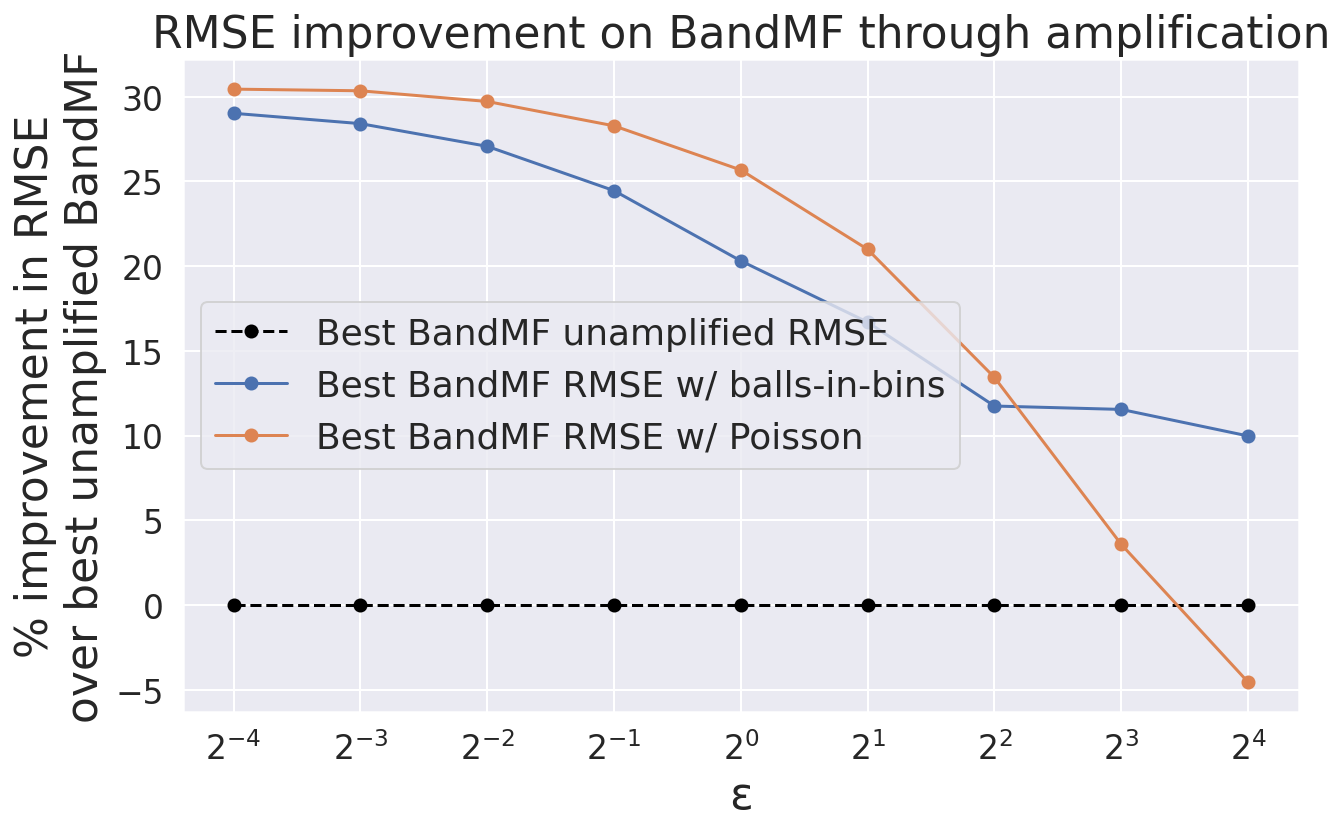
\includegraphics[width=0.95\linewidth]{other_figures/improvement-on-best-band-mf.png}
    \caption{Improvement in RMSE over unamplified $b$-banded matrix factorization due to different amplification schemes. All curves optimize the choice of $b$ at each point.}
    \label{fig:improvement-on-variable-bandmf}
    \end{subfigure}
    \begin{subfigure}{.05\textwidth}
    \end{subfigure}
    \begin{subfigure}{.45\textwidth}
    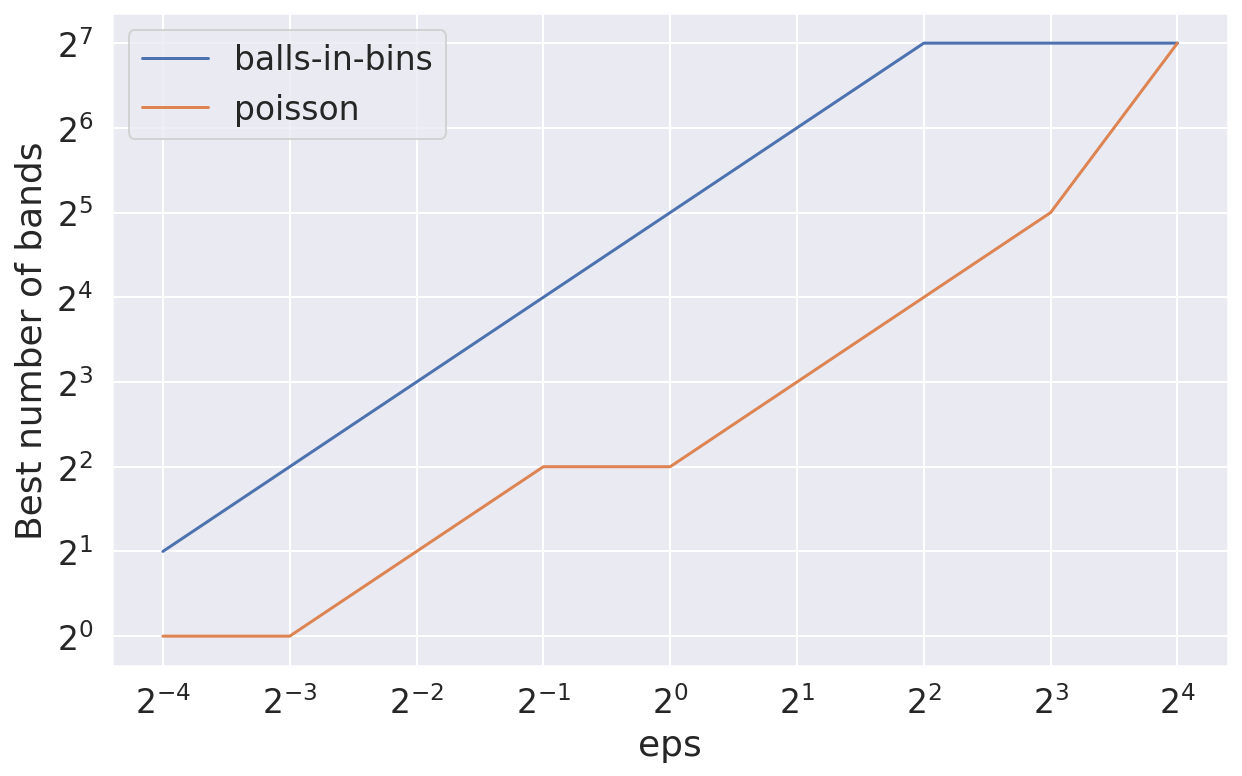
\includegraphics[width=0.95\linewidth]{other_figures/best_band_choice.png}
    \caption{For each of the amplification methods in Figure~\ref{fig:improvement-on-variable-bandmf}, the best choice of $b$ at each value of $\varepsilon$.}
    \label{fig:best_band_choice}
    \end{subfigure}
    \begin{subfigure}{.45\textwidth}
    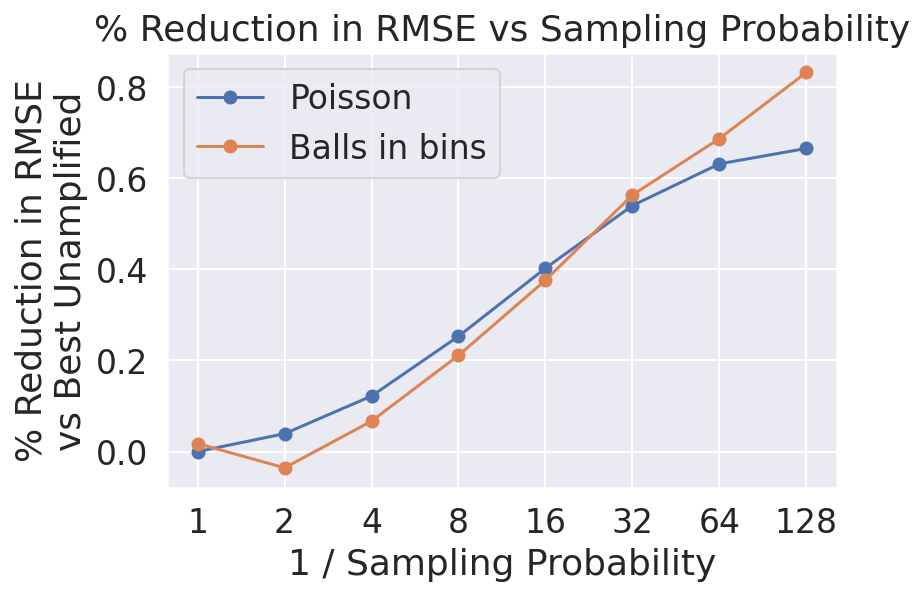
\includegraphics[width=0.95\linewidth]{other_figures/rmse_vs_prob.png}
    \caption{Comparison of improvement due to amplification as a function of sampling probability.}
    \label{fig:rmse_vs_prob}
    \end{subfigure}
    \begin{subfigure}{.05\textwidth}
    \end{subfigure}
    \begin{subfigure}{.45\textwidth}
    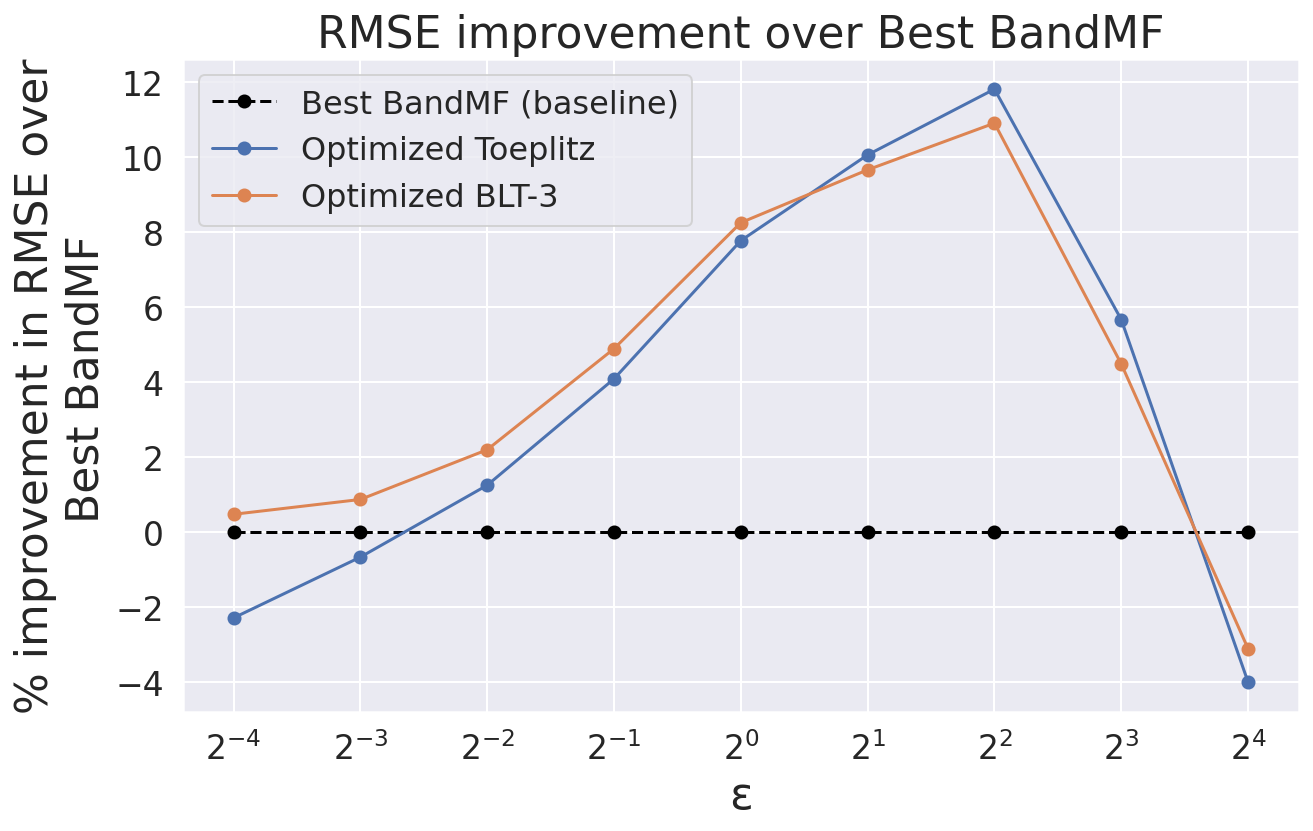
\includegraphics[width=.95\linewidth]{other_figures/improvement-on-best-band-mf-amp.png}
    \caption{Improvement from optimizing $\bfC$ using objective accounting for amplification.}
    \label{fig:rmse_over_amplified_bandmf}
    \end{subfigure}
    \caption{Comparisons for variable $\bfC$.}
\end{figure}

For $\eps \leq 4$, the best RMSE under Poisson sampling slightly outperforms balls-in-bins batching and for $\eps \geq 8$, we see a deterioration in the RMSE improvements from Poisson. At $\epsilon = 16$, we see that it is better to forgo the amplification scheme of \citep{choquette2024amplified} and use the unamplified baseline. In contrast, because the distinguishing problem for balls-in-bins for a fixed $\bfC$ is always strictly harder than the unamplified baseline, the best $\bfC$ combined with balls-in-bins batching always strictly improves over the unamplified baseline. 

\subsubsection{Improvements due to optimization}

We now look at the benefits of using our optimization procedure to choose $\bfC$. We compare two variants of our optimization scheme, one which optimizes over general Toeplitz matrices, and another which optimizes over the BLT matrix family defined by \citet{dvijotham2024efficientnearoptimalnoisegeneration}. We use the 3-buffer variant of BLTs, i.e. they can be specified using 6 parameters and only require an overhead of 3 times the model size to store the state required for correlated noise generation. In Figure~\ref{fig:rmse_over_amplified_bandmf} we plot the improvement in RMSE for both these variants relative to the best $b$-banded $\bfC$ amplified using the sampling scheme and analysis of \citet{choquette2024amplified}. 

We observe that for most $\epsilon$ values, our optimization procedure for $\bfC$ can give a reduction in RMSE compared to the previous state-of-the-art of \citet{choquette2024amplified}. For extreme values of $\epsilon$, the banded baseline still outperforms our optimized matrices. We note that despite BLT matrices being a subset of Toeplitz matrices, our optimized BLTs matrices sometimes outperform our optimized Toeplitz matrices. We believe this is because BLTs lie in a lower-dimensional space which may make it easier to optimize over them, i.e. the suboptimality of our solution to the optimization problem over BLTs may be smaller than the suboptimality of our solution to the problem over Toeplitz matrices.


\subsubsection{Timing Analysis}

In this section, to understand the scalability of our optimization procedure, we analyze how long it takes to optimize for the matrix $\bfC$ as well and how it depends on the various parameters.

In Figure~\ref{fig:timing-table}, we give the time, in seconds, for completing 300 iterations of gradient descent while varying the number of epochs, iterations per epoch, and number of samples per gradient descent iteration. We use a v100 GPU to perform the gradient steps. Here we fix $\delta = 10^{-5}$ and $\eps=1$. We make the following observations:
\begin{itemize}
    \item Increasing the number of samples multiplicatively by 8 does not cause the runtime to increase by the same amount.
    \item On average, the runtime seems to have a sublinear dependence in the number of epochs.
    \item In contrast, in most settings for a large enough number of iterations per epoch the runtime seems to grow linearly or worse in the iterations per epoch.
\end{itemize}

For the largest number of samples, epochs, and iterations per epoch we ran into memory issues. In the next section, we show that using a very small number of samples in the optimization loop still yields good RMSE, i.e. these memory issues can generally be avoided. Combined with these observations, we believe this is evidence the optimization procedure is scalable in the number of epochs, although it may be infeasible to run the procedure for a large number of iterations per epoch.

\begin{figure}
    \centering
\begin{tabular}{cllll}
\toprule
\multicolumn{5}{c}{Number of Samples = 131072} \\
\hline
\multicolumn{1}{l}{} & \multicolumn{1}{l|}{} & \multicolumn{3}{c}{Number of Epochs} \\
\cline{3-5} 
\multicolumn{1}{l}{} & \multicolumn{1}{l|}{}
  & 16 & 32 & 64 \\
\hline
\multicolumn{1}{c|}{\multirow{3}{*}{\begin{tabular}[c]{@{}c@{}}
Iterations\\ per epoch\end{tabular}}}
& \multicolumn{1}{l|}{32}  & 376.88 & 384.44 & 311.55 \\
\multicolumn{1}{c|}{} &
\multicolumn{1}{l|}{64}  & 383.19 & 323.56 & 658.95 \\
\multicolumn{1}{c|}{}
& \multicolumn{1}{l|}{128} & 389.37 & 770.18 & 3594.55  \\
\bottomrule
\end{tabular}
\begin{tabular}{cllll}
\toprule
\multicolumn{5}{c}{Number of Samples = 1048576} \\
\hline
\multicolumn{1}{l}{} & \multicolumn{1}{l|}{} & \multicolumn{3}{c}{Number of Epochs} \\
\cline{3-5} 
\multicolumn{1}{l}{} & \multicolumn{1}{l|}{}
  & 16 & 32 & 64 \\
\hline
\multicolumn{1}{c|}{\multirow{3}{*}{\begin{tabular}[c]{@{}c@{}}
Iterations\\ per epoch\end{tabular}}}
& \multicolumn{1}{l|}{32}  & 374.33 & 394.50 & 468.48 \\
\multicolumn{1}{c|}{} &
\multicolumn{1}{l|}{64}  & 525.25 & 664.23 & 804.56 \\
\multicolumn{1}{c|}{}
& \multicolumn{1}{l|}{128} & 1060.45 & 1435.47 & Out of memory \\
\bottomrule
\end{tabular}
\caption{Time (in seconds) to optimize $\bfC$ for different values of Monte Carlo samples used per gradient descent iteration, number of epochs, and iterations per epoch.}
\label{fig:timing-table}
\end{figure}

\subsubsection{Effect of the number of samples}
When optimizing over the matrix $\bfC$, we use a Monte Carlo sampler to estimate $\sigma$. However, for privacy purposes we only need the estimate of $\sigma$ to be accurate for the final $\bfC$ output by the optimization procedure, since that is the only correlation matrix we will actually use during model training. For intermediate values of $\bfC$ in the gradient descent procedure, it is not a privacy violation to compute inaccurate $\sigma$ values for these matrices.

In turn, to make the optimization procedure more efficient, we can use a smaller number of samples per iteration. A natural question is then if the number of samples needed for the Monte Carlo estimator to concentrate is comparable to the number of samples needed for the optimization to achieve reasonable RMSE.

We run our optimization procedure for a varying number of samples per iteration, and in \cref{fig:optimization-samples} for each of these numbers we plot the suboptimality of the final $\bfC$ value in terms of RMSE achieved compared to using the maximum number of samples. We vary $\epsilon$ and fix $\delta = 10^{-5}$. For this choice of $\delta$, we need at least $1/\delta \approx 2^{17}$ samples are needed for the Monte Carlo estimator of $\delta$ to guarantee an error smaller than $\delta$ with, say, constant probability. However, in Figure~\ref{fig:optimization-samples}, we see that for $\epsilon = 0.5, 1, 2$ using e.g. $\approx 2^9$ samples per iteration suffices for achieving similar RMSE as $2^{20}$ samples per iteration, and at $\epsilon = 4$ this number of samples only leads to a $\approx 10\%$ increase in RMSE. In other words, our optimization procedure can use a much smaller number of samples (compared to the final verification of $\bfC$ and $\sigma$) at little to no cost in utility.

\begin{figure}[h]
    \centering
    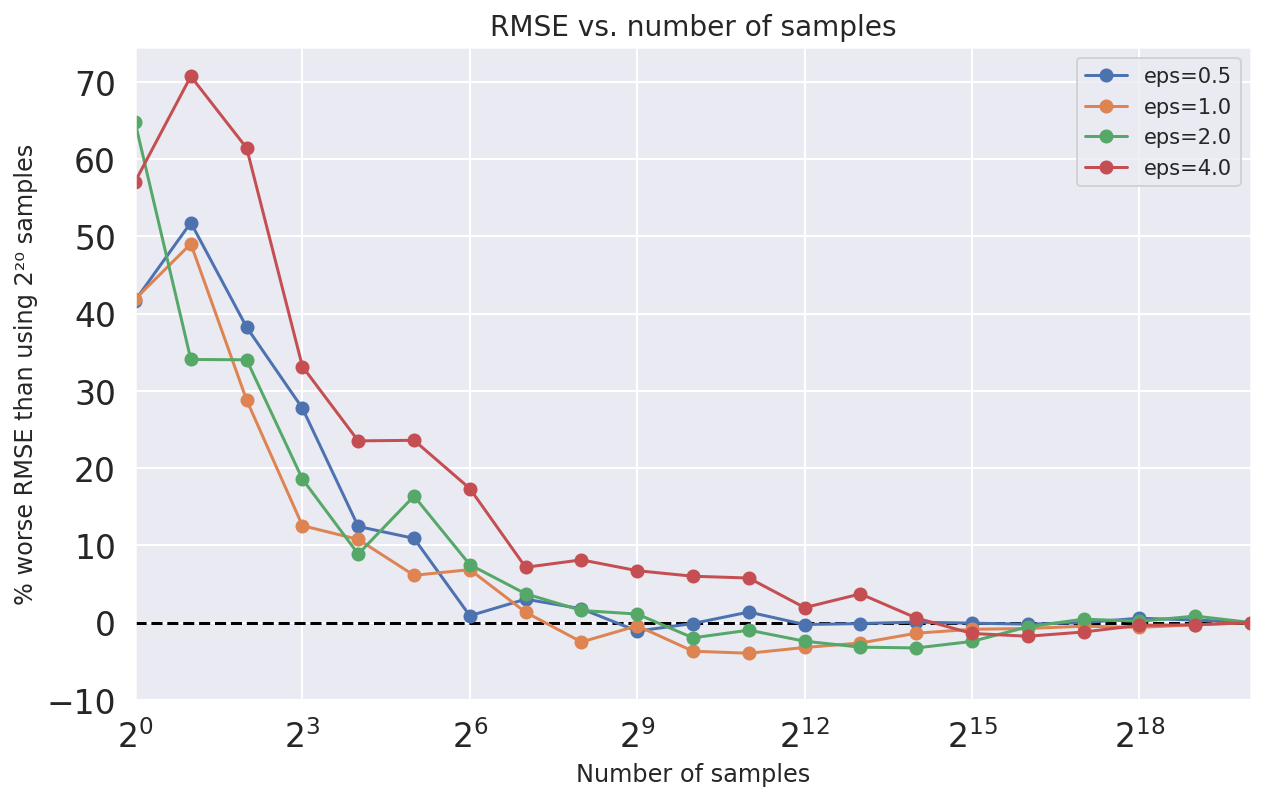
\includegraphics[width=0.95\textwidth]{num-samples-plots/rmse_vs_numsamples.png}
    \caption{Percentage increase in RMSE due to using a smaller number of samples per iteration in the optimization procedure, when compared to the RMSE achieved by using $2^{20}$ samples per iteration.}
    \label{fig:optimization-samples}
\end{figure}

\subsection{CIFAR Results}\label{sec:cifar}

We next compare different choices of the correlation matrix $\bfC$ and amplification schemes in a deep learning setting. We replicate the CIFAR10 image recognition setting considered by  \citep{choquette2024amplified}: we also use the same VGG model, 20 epochs of 100 iterations with batch size 500, and momentum of 0.95 and a learning rate cooldown from $\eta$ to $\eta/20$ across iterations 500 to 2000. We vary $\epsilon \in \{0.5, 1.0, 2.0, 4.0, 8.0\}$ and fix $\delta = 10^{-5} < 1/|D|$. We fix the clip norm to 1.0 and tune the learning rate separately for each combination of $\epsilon$ and correlation matrix/amplification method, and then report the average of 100 training runs for each combination. The different correlation matrix choices and amplification methods we consider are:

\begin{itemize}
    \item Our baseline is the SOTA of banded matrices of \citet{choquette2024amplified} using their Poisson sampling-based amplification scheme. We also consider banded matrices and balls-in-bins batching. Following \citet{choquette2024amplified}, for each choice of the number of bands $b$, we optimize $\bfC$ without accounting for amplification. Then for each amplification method, we use the choice of $b$ in each setting of $\epsilon$ that gives the lowest RMSE under amplification.
    \begin{itemize}
        \item We do not separately consider multi-epoch MEMF of \citet{choquette2022multi} or DP-SGD with Poisson sampling as they are subsumed by this approach.
    \end{itemize}
    \item BLT matrices of \citet{dvijotham2024efficientnearoptimalnoisegeneration}. We restrict to 4 buffers and use our optimization framework to optimize $\bfC$ for the RMSE under balls-in-bins batching for each value of $\epsilon$.
    \item General Toeplitz lower-triangular matrices. Again we use our optimization framework to optimize $\bfC$ for the RMSE under balls-in-bins batching for each value of $\epsilon$.
\end{itemize}


For all methods, in the implementation we shuffle the dataset and use a fixed batch size, but calculate the noise multiplier assuming the corresponding amplification method was properly implemented. 
This is a standard practice for simplifying implementations in the literature (e.g., \citet{choquette2024amplified}). In the next section we discuss the pitfalls of this practice, and do a training run where we actually implement a practical variant of balls-in-bins batching that also uses fixed batch sizes for gradient computations.
\begin{figure}
    \centering
    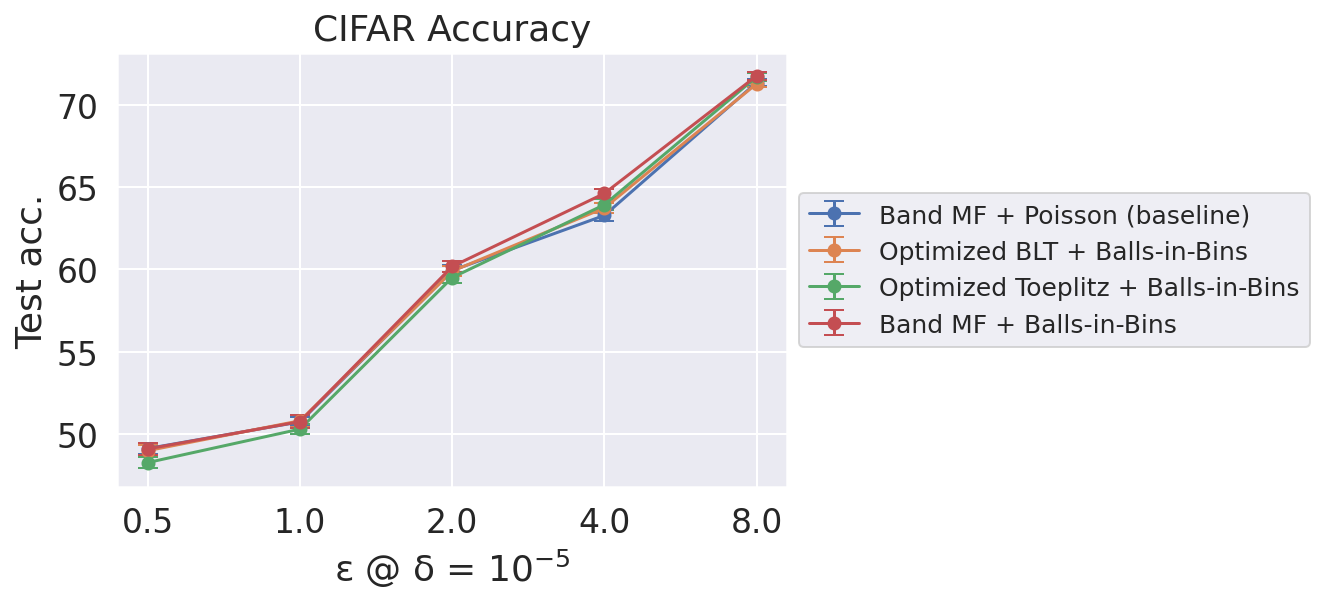
\includegraphics[width=0.95\textwidth]{cifarplots/cifar_amplification_unnormalized.png}
    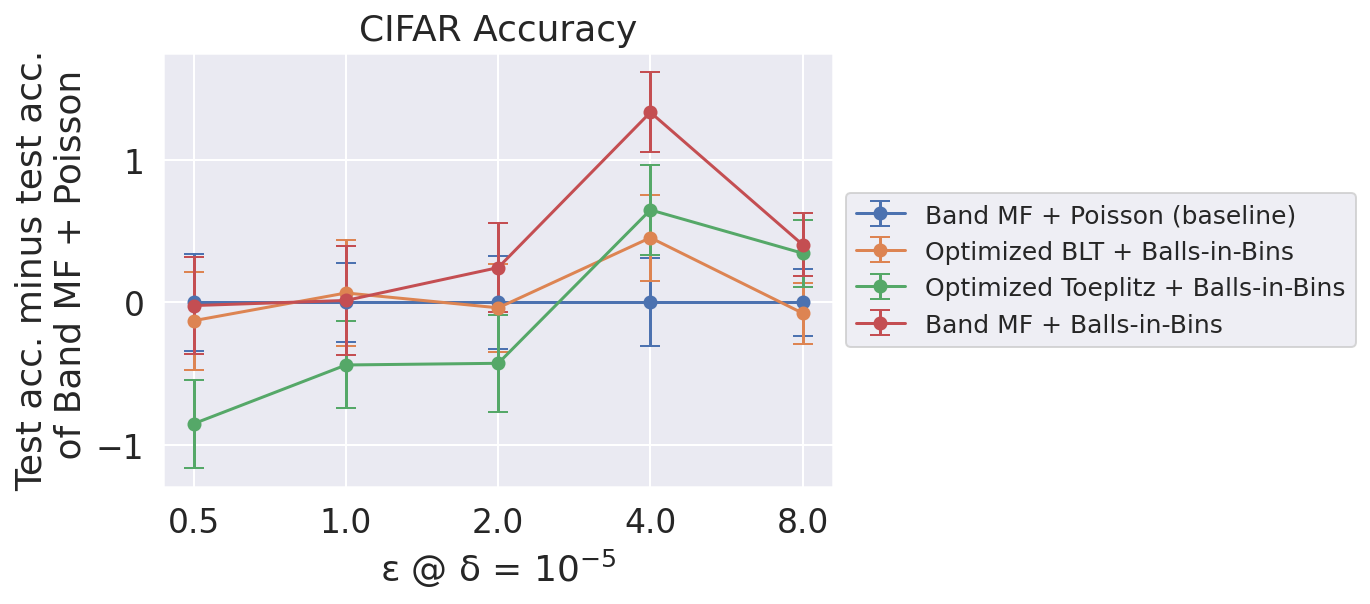
\includegraphics[width=0.95\linewidth]{cifarplots/cifar_amplification.png}
    \caption{Comparison of accuracy on CIFAR of different correlated noise strategies and amplification methods, absolute and relative to the baseline of banded $\bfC$ + Poisson sampling, with 95\% confidence intervals over 100 trials. }
    \label{fig:cifar_accuracies}
\end{figure}

In~\cref{fig:cifar_accuracies}, we plot the test accuracy achieved by each combination of correlation matrix and amplification analysis. We can conclude the following:

\begin{itemize}
    \item\emph{Banded matrix factorization + balls-in-bins} is always at least as good as the baseline, and sometimes gives up to 1\% accuracy improvements. As argued earlier, the baseline assumes Poisson sampling which is a stronger/less practical assumption. 
    \item Our ability to optimize BLT matrices makes them also always at least as good as the baseline, but with smaller improvements than the previous bullet. The baseline uses up to $16$ bands depending on $\epsilon$, so~\emph{BLTs are also up to 4x more memory efficient than the baseline}.
    \item Optimized Toeplitz matrices are incomparable to the baseline; we believe their weak performance relative to the other methods is due to the difficulty of the optimization problem. 
\end{itemize}


\begin{figure}
\begin{center}
\begin{tabular}{|c|c|c|c|c|c|}
\hline
 Method / $\epsilon$ & 0.5 & 1.0 & 2.0 & 4.0 & 8.0 \\ 
 \hline
 BandMF + Poisson & 1.018 & 0.778 & 0.606 & 0.481 & 0.388 \\  
 \hline
 BandMF + Balls-in-Bins & 2.829 & 2.071 & 1.455 & 0.802 & 0.470\\  
 \hline
 Optimized BLT + Balls-in-Bins & 2.609 & 1.598 & 1.079 & 0.694 & 0.448 \\  
 \hline
 Optimized Toeplitz + Balls-in-Bins & 2.003 & 1.182 & 0.864 & 0.639 & 0.445 \\  
 \hline
\end{tabular}
\end{center}
\caption{Noise multiplier $\sigma$ used in the CIFAR10 experiments for different correlated noise strategies and amplification methods. Note that different strategies which have higher noise cancellation require higher $\sigma$, so a lower noise multiplier alone does not imply better learning performance.}
\end{figure}

\begin{figure}
\begin{center}
\begin{tabular}{|c|c|c|c|c|c|}
\hline
 Method / $\epsilon$ & 0.5 & 1.0 & 2.0 & 4.0 & 8.0 \\ 
 \hline
 BandMF + Poisson & 2 & 4 & 8 & 16 & 32 \\  
 \hline
 BandMF + Balls-in-Bins & 16 & 32 & 64 & 64 & 64\\  
 \hline
\end{tabular}
\end{center}
\caption{Number of bands used in the CIFAR10 experiments for BandMF combined with different amplification methods.}
\end{figure}



\subsubsection{Practical Implementation of Balls-in-Bins Batching}\label{sec:practical}

In Section~\ref{sec:cifar}, and in most empirical research on DP model training, an amplification method like Poisson sampling is assumed when computing the noise multiplier, but for simplicity a simpler sampling scheme is not actually implemented. The most common case of this is assuming Poisson sampling when instead doing shuffling, even though shuffling can produce much larger $\epsilon$ values than sampling \citep{chua2024private}. A notable exception is research built on Opacus~\citep{opacus} which implements Poisson sampling.

The main issue with implementing such sampling schemes properly is that they usually lead to unequal batch sizes (as schemes like shuffling which enforce equal batch sizes are usually hard to analyze tightly), which can lead to several inefficiencies:

\begin{itemize}
    \item Modern model training pipelines are optimized for a fixed batch size. For example, XLA, which is used to e.g. compile gradient computations implemented in libraries like TensorFlow and JAX, requires a static input shape. To use variable batch sizes, one would naively need to forgo the use of XLA which could heavily slow down training in large-scale settings.
    \begin{itemize}
        \item For example, consider Opacus which correctly implements Poisson sampling and supports variable batch sizes. In the benchmarking experiments of \citep{opacus}, Opacus was shown to have runtime competitive with JAX for small-scale DP training. However, they observed that e.g. JAX pays a large up-front cost for compilation but after compilation achieves better runtime per iteration than Opacus. We expect that for larger scale the training the time spent on compilation is a smaller fraction of training time, hence variable batch size training with Opacus would be less scalable than XLA-based training using fixed batch sizes.
    \end{itemize}
    \item Sampling a slightly larger batch can lead to disproportionately longer gradient computation times. As an extreme case, suppose we use an expected batch size of $B$, and we have $B$ accelerators that can each process a single gradient in parallel in time $T$. Hence computing a batch gradient on $B$ examples takes time $T$. However, if we have $B+1$ samples instead, we will need time $2T$ instead.
    \item Sampling a smaller batch leads to wasted computational resources. For example, in the above setting, if we sampled $9B/10$ examples, then we would have $B/10$ accelerators being unused, which may be undesirable.
\end{itemize}

To this end we propose and implement a practical variant of balls-in-bins batching. We do balls-in-bins batching, but:
\begin{itemize}
    \item If a batch has size less than $B$, we pad it with some examples that have gradient 0 so its batch size becomes $B$.
    \item If a batch has size greater than $B$, we truncate it to have size exactly $B$.
    \item We compute the average gradient over the padded/truncated batch (i.e. our normalization in the average is always $1/B$).
\end{itemize}

Recall that balls-in-bins (without padding and truncating) can be implemented by shuffling the dataset, sampling a batch size schedule, and then taking batches according to this schedule. Hence even with padding and truncating balls-in-bins requires minimal overhead on top of shuffling, and indeed we were easily able to implement it in our CIFAR training code using only a single shuffle on the dataset and \texttt{numpy}'s multinomial sampler and pad operations, and use XLA to compile gradient computations in the resulting code. Furthermore, none of these changes affects the privacy analysis. This is because (i) the fixed normalization is compatible with the privacy analysis which is implicitly analyzing at the sum rather than the average, (ii) truncating a batch is equivalent to some of the examples in that batch having gradient 0, and DP-SGD's privacy analysis allows arbitrary clipped gradient.

We next demonstrate that the loss in utility due to truncating examples or not saturating the batch size in every iteration is acceptable. We rerun the training procedure from the previous section using BLT matrices (we focus on BLT matrices as they are the most scalable choice of correlated noise \citep{mcmahan2024hasslefreealgorithmprivatelearning}), but implement our practical variant of balls-in-bins batching. We pad/truncate to the same batch size of 500, i.e. in terms of gradient computations our practical variant of balls-in-bins is no more costly than shuffling the dataset and using fixed batch sizes instead. 

In Figure~\ref{fig:implementation} we compare this implementation to (i) the same implementation but using shuffling instead of balls-in-bins batching, and (ii) the state-of-the-art unamplified baseline of MEMF.
We see that \textit{the improvements from amplification over the unamplified baseline are far larger than the loss in utility due to the suboptimal batching introduced by the sampling scheme}. To the best of our knowledge, this is the first DP model training result that simultaneously (i) implements the sampling scheme assumed when computing the noise multiplier, (ii) does so at a negligible cost in efficiency and in a manner compatible with modern machine learning frameworks, and (iii) still demonstrates improvements over the unamplified baseline.

\begin{figure}
    \centering
    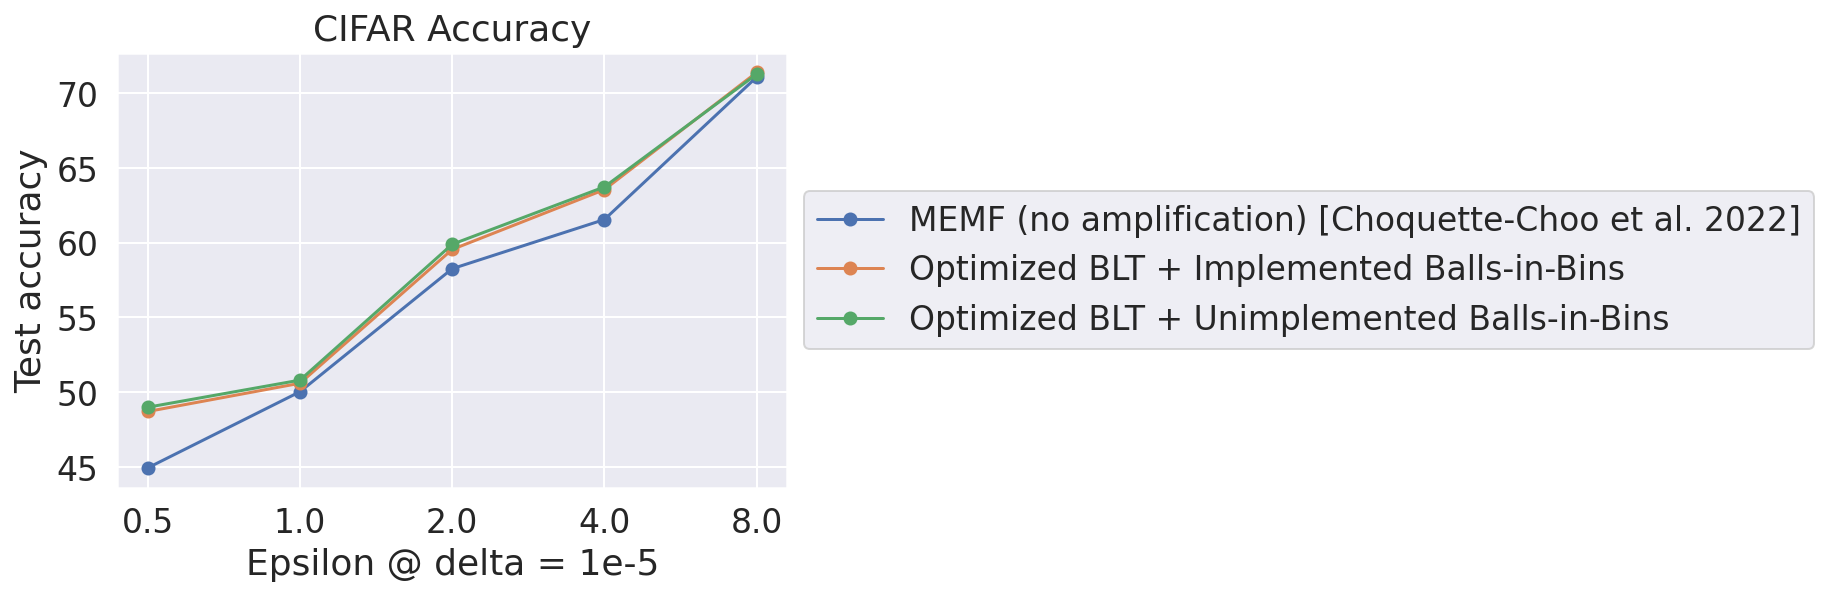
\includegraphics[width=0.95\linewidth]{cifarplots/implementation.png}
    \caption{Comparison of implementing balls-in-bins batching to shuffling and assuming balls-in-bins in the analysis, and the unamplified baseline.}
    \label{fig:implementation}
\end{figure}